\documentclass[../main.tex]{subfiles}

\begin{document} %%%%%%%%%%%%%%%%%%%%%%%%%%%%%%%%%%%%%%%%%%%%%%%%%%%%%%%%%%%%
\section{Semana 1} 
    \subsection{Alineación y Padding}
        La alineación y el padding son técnicas utilizadas por el compilador para optimizar el acceso a la memoria y mejorar el rendimiento del programa. 
        
        La \textbf{alineación} se refiere a la forma en que se almacenan los datos en la memoria, asegurándose de que los datos se almacenen en direcciones de memoria múltiplos de cierto tamaño (generalmente 4 bytes) Ver \cite{Alineación}. El \textbf{padding} se refiere a la inserción de bytes adicionales en la memoria para asegurar que los datos estén alineados correctamente. Aunque la alineación y el padding pueden mejorar el rendimiento del programa, también pueden desperdiciar memoria.
    
        % Cargamos una imagen
        \begin{figure}[htbp]
            \centering
            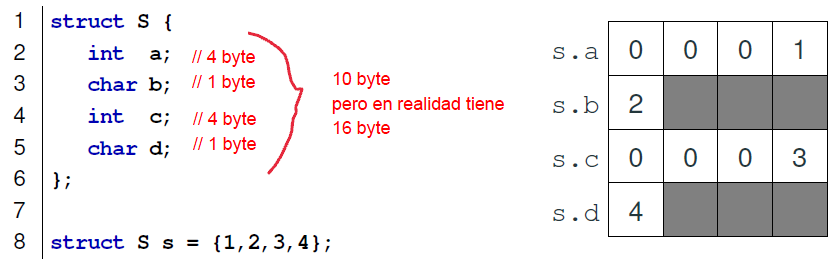
\includegraphics[width=0.8\textwidth]{../images/alineacion_padding.png}
            \caption{Alineación y Padding}
            \label{fig:alineacion}
        \end{figure}

        En la figura anterior se genera una ALINEACION (predefinida de 4 bytes),entre variables, y se agrega un PADDING de 3 bytes para las variables char. \\

        \underline{Caracteristicas:}
        \begin{enumerate}
            \item El compilador puede guardar las variables en posiciones de memoria múltiplos de 4 (depende de la arquitectura y de los flags de compilación): variables alineadas son accedidas más rápidamente que las desalineadas.
            \item Como contra, la alineación despedicia espacio (padding) hay un tradeoff entre velocidad y espacio.
            \item El padding se hace mas notorio en las estructuras: el acceso a cada atributo es rápido pero hay memoria desperdiciada.
        \end{enumerate}

    \subsection{Endianess}
        El término inglés endianness ("extremidad") designa el formato en el que se almacenan los datos de más de un byte en un ordenador. El problema es similar a los idiomas en los que se escriben de derecha a izquierda, como el árabe, o el hebreo, frente a los que se escriben de izquierda a derecha, pero trasladado de la escritura al almacenamiento en memoria de los bytes.


        \begin{itemize}
            \item sistema \textbf{big-endian}: consiste en representar los bytes en el orden "natural". Primer byte es el *mas* significativo.
                \begin{equation*}
                    \text{0x12345678} \rightarrow \text{\{0x12, 0x34, 0x56, 0x78\}}                        
                \end{equation*}
            \item sistema \textbf{little-endian}: consiste en representar los bytes en el orden inverso al "natural". Primer byte es el *menos* significativo (LINUX MINT)
                \begin{equation*}
                    \text{0x12345678} \rightarrow \text{\{0x78, 0x56, 0x34, 0x12\}}                        
                \end{equation*}
        \end{itemize}

    \subsection{Cache friendly}
        Cache friendly se refiere a una técnica de programación que busca optimizar el acceso a la memoria caché de la CPU para mejorar el rendimiento de un programa.

        La memoria caché es una memoria de acceso rápido que se utiliza para almacenar temporalmente los datos que se utilizan con frecuencia en un programa. La CPU accede a la memoria caché mucho más rápido que a la memoria principal, por lo que si los datos que necesita están en la caché, el programa se ejecutará más rápido.
        
        La técnica de programación cache friendly busca organizar los datos en la memoria de tal manera que se maximice la probabilidad de que los datos que se necesitan estén en la caché. Esto se puede lograr de varias maneras, como por ejemplo:
        
        \begin{itemize}
            \item Utilizar arreglos en lugar de punteros: los arreglos son más eficientes que los punteros porque los datos están almacenados de manera contigua en la memoria, lo que facilita el acceso a la caché.
            \item Utilizar arreglos de estructuras en lugar de estructuras de arreglos: los arreglos de estructuras son más eficientes que las estructuras de arreglos porque los datos están almacenados de manera contigua en la memoria, lo que facilita el acceso a la caché.
            \item Utilizar estructuras de datos que minimicen la fragmentación de la memoria: la fragmentación de la memoria puede hacer que los datos estén dispersos en la memoria, lo que dificulta el acceso a la caché.
            \item Utilizar algoritmos que accedan a los datos de manera secuencial: los algoritmos que acceden a los datos de manera secuencial son más eficientes que los que acceden a los datos de manera aleatoria porque facilitan el acceso a la caché.
        \end{itemize}

    \subsection{Onboarding - Recap 01 - Proceso de Building y Testing}
        Building = contruccióm y testing = pruebas.\\


    \subsection{Conceptos}
        
        Un \textbf{linter} es una herramienta de software diseñada para analizar el código fuente de programas y detectar posibles errores, problemas de estilo y prácticas no recomendadas en el código. Su objetivo es mejorar la calidad del código y facilitar el mantenimiento y la colaboración en proyectos de desarrollo de software.

        Los linters funcionan revisando el código en busca de patrones específicos que podrían indicar problemas. Estos patrones pueden incluir desde errores de sintaxis obvios hasta recomendaciones de estilo, como la indentación adecuada, el uso consistente de nombres de variables y funciones, la ausencia de variables no utilizadas y mucho más.

        Los linters se enfocan en inconsistencias de estilos en el código, también errores lógicos potenciales y, a menudo, sugieren soluciones para el código.


        Los \textbf{static checkers} (verificadores estáticos) son herramientas de análisis estático de código que examinan el código fuente de un programa sin ejecutarlo. A diferencia de los verificadores dinámicos, que evalúan el comportamiento del programa durante la ejecución, los verificadores estáticos se centran en inspeccionar el código en busca de posibles problemas, errores y violaciones de reglas antes de que el programa se ejecute.

        Estos verificadores realizan análisis estáticos exhaustivos, como revisar la estructura del código, la sintaxis, la semántica y el flujo de control, con el fin de identificar problemas potenciales. A menudo, se utilizan para encontrar errores comunes y detectar problemas de seguridad, convenciones de estilo y prácticas recomendadas.
        
        Algunos ejemplos de verificadores estáticos son:

        cpplint y cppcheck son dos herramientas de análisis estático para código C++12.
        \begin{itemize}
            \item \textbf{cpplint} es una herramienta de línea de comandos para verificar si los archivos C/C++ cumplen con la guía de estilo de C++ de Google1. Está desarrollado y mantenido por Google Inc. en google/styleguide1. 
            \item \textbf{cppcheck} es una herramienta de análisis estático para código C/C++ que detecta principalmente tipos de errores que los compiladores normalmente no detectan. Su objetivo es detectar solo errores reales en el código (es decir, tener cero falsos positivos).
        \end{itemize}



    \subsection{Erroes de compilación}
        gcc -Wall -Werror -std=c11 -pedantic -c  01\_simple.c
        \begin{itemize}
            \item \textbf{-Wall:} emitir todos los warnings
            \item \textbf{-Werror:} todos los warnings son considerados errores (detienen el proceso)
            \item \textbf{-std=c11:} ser estricto y no permitir nada fuera del estandar C11
            \item \textbf{-pedantic:} ser mas estrictos con el estandar
            \item \textbf{-c:} gcc detiene el proceso luego de la etapa de compilacion
            \item \textbf{-o:} gcc -o 01\_simple 01\_simple.c
            \item \textbf{-static:} fuerza a que el linkeo sea estatico, agregando el codigo objeto al binario final
            \item \textbf{-fPIC:} el codigo generado no asume posiciones fijas en memoria sino relativas a una posicion "a definir". Este nivel de indireccion es representado por la estructura GOT (global offset table) que es completada al momento que un ejecutable carga la libreria dinamica.
            \item \textbf{-shared:} genera una libreria dinamica que puede ser cargada en un ejecutable en tiempo de load (cuando el programa se carga a memoria) o incluso en tiempo de ejecucion (el mismo programa que ya esta corriendo puede cargar esta libreria)
            \item \textbf{-ldl:} Carga la libreria dl necesaria con las definiciones de las funciones dlopen, dlsym, dlerror y dlclose entre otras. Dichas funciones nos permitiran cargar una libreria dinamica en tiempo de ejecucion.
            
        \end{itemize}
        
        objdump -d 01\_simple.o
        \begin{itemize}
            \item \textbf{-d:}desensambla (disassembly): intenta tomar el codigo objeto (binario)y traducirlo a codigo assembly, ligeramente mas entendible para el humano.
        \end{itemize}



        gcc -Wall -Werror -std=c11 -pedantic -ggdb -c 01\_simple.c
        \begin{itemize}
            \item \textbf{-ggdb:} incluye en el binario todos los simbolos y datos necesarios para poder correlacionar el codigo objeto con el codigo fuente y asi poder debuggear
        \end{itemize}

    \subsection{Buffer overflow, Segmentation fault}
        Un segmentation fault se da cuando un proceso intenta realizar una operación para la que no tiene permisos sobre un segmento de memoria. Es común ver un segmentation fault cuando se intenta desreferenciar un puntero nulo. Para clarificar la parte de los permisos, también recibiríamos un segmentation fault si intentamos escribir al code-segment, mientras que no sucede si lo leemos, porque tenemos permiso de sólo lectura.

        Un buffer overflow es acceder a memoria contigua a la asignada para cierta variable. Usualmente pasa cuando escribimos más allá de los límites de algún arreglo de memoria, pisando o leyendo memoria contigua. \href{https://taller-de-programacion.github.io/blog/2021/04/26/SIGSEGV-BufOverflow.html}{link}







































\end{document}  %%%%%%%%%%%%%%%%%%%%%%%%%%%%%%%%%%%%%%%%%%%%%%%%%%%%%%%%%%%%%
